% !TeX document-id = {1700c40c-d810-430a-9d0b-2789b57637de}
% !TeX TXS-program:compile = txs:///pdflatex/[--shell-escape]

\documentclass[11pt, letterpaper]{article}

\usepackage[utf8]{inputenc}
\usepackage[T1]{fontenc}
\usepackage{lmodern}
\usepackage{graphicx}
\usepackage{longtable}
\usepackage{wrapfig}
\usepackage{rotating}
\usepackage{amsmath}
\usepackage{textcomp}
\usepackage{amssymb}
\usepackage{hyperref}
\usepackage{minted}
\usepackage[spanish]{babel}
\usepackage[round]{natbib}
\usepackage{logicproof}
\usepackage{enumerate}%

\title{\textsc{Representación del conocimiento} \\
	Tarea 5
}  

\author{Angel García Báez\\
	Alumno de la Maestría en Inteligencia Artificial \\ \\ \textbf{IIIA}
	Instituto de Investigaciones en Inteligencia Artificial \\
	Universidad Veracruzana \\ \emph{Campus Sur, Calle Paseo Lote II,
		Sección 2a, No 112} \\ \emph{Nuevo Xalapa, Xalapa, Ver., México 91097}
	\\ \\ ZS24019400@estudiantes.uv.mx}

\date{\today}


\begin{document}
	
\maketitle

\newpage
	
\section{Creación de una ontología en protégé}
	
\textbf{Con la ayuda del tutorial de Michael DeBellis, A Practical Guide to Building
	OWL Ontologies Using Protégé 5.5 and Plugis (edition 3.2, 8 october 2021),
	realise los siguientes ejercicios:}
		
	

\subsection{Con base en la base de conocimientos del Covid-19 que implementaron en su tarea 3, implemente una Ontología equivalente en Protégé. [50]}

Retomando el trabajo hecho en la tarea 3 de implementar un pseudo-sistema experto en prolog y diseñando la base del conocimiento obtenida de los lineamientos del manual de Covid-19. Si bien, el paradigma sigue siendo la representación del conocimiento, cambian un poco las reglas del juego al necesitar implementar clases, sub-clases, relaciones y propiedades con  otro estilo que no sea el de prolog. 

Antes de siquiera empezar a trabajar con protégé, es necesario identificar los elementos que ya tengo y empezar a re-pensarlos en términos de la ontología, por lo que  a continuación hago un desglose de lo que ya tengo, pero en terminos que me funcionan mejor para hacer el cambio de una cosa a otra:

Tengo las clases principales:

\begin{itemize}
	\item Persona
	\item Personal de salud
	\item Enfermera que es sub clase de personal de salud
	\item Epidemiologo que es sub clase de personal de salud
	\item Síntoma
	\item Precaución
	\item PrecauciónEstandar que es sub clase de Precaución
	\item PrecauciónGotas que es sub clase de Precaución
	\item PrecauciónAerosoles que es sub clase de Precaución
	\item TipoDeMuestra
	\item Pais
	\item Pais de riesgo que es un subtipo de pais
	\item Nivel de Atención
	\item Tipo de aislamiento
	\item Caso
	\item CasoSospechoso que es subtipo de Caso
	\item CasoConfirmado que es subtipo de Caso
	
\end{itemize}

Posteriormente, se definen algunas propiedades (que son las relaciones entre las entidades):

\begin{itemize}
	\item presentaSintoma: va de Persona a Sintoma.
	\item tieneEnfermedadRespiratoria: va de Persona a Enfermedad.
	\item viajoA: va de Persona a Pais (o PaisDeRiesgo).
	\item contactoCon: va de Persona a Persona.
	\item resultadoLaboratorio: va de Persona a ResultadoLaboratorio.
	\item aplica: va de PersonalDeSalud a Precaucion.
	\item tomaMuestra: va de PersonalDeSalud a TipoDeMuestra.
	\item aislamientoRecomendado: va de Persona a TipoAislamiento.
	\item nivelAtencion: va de Persona a NivelAtencion.
	
\end{itemize}

Posteriormente, se muestran las instancias declaradas dentro de la ontología.


\begin{itemize}
	\item juan que es una instancia de Persona.
	\item maria que es una instancia de Persona.
	\item pedro que es una instancia de Persona.
	\item enfermera1 que es una instancia de Enfermera.
	\item epidemio1 que es una instancia de Epidemiologo.
	\item china que es una instancia de PaisDeRiesgo.
	\item italia que es una instancia de PaisDeRiesgo.
	\item iran que es una instancia de PaisDeRiesgo.
	\item japon que es una instancia de PaisDeRiesgo.
	\item hong kong que es una instancia de PaisDeRiesgo.
	\item corea del sur que es una instancia de PaisDeRiesgo.
	\item singapur que es una instancia de PaisDeRiesgo.
	\item fiebre que es una instancia de Sintoma.
	\item tos que es una instancia de Sintoma.
	\item dificultad respiratoria que es una instancia de Sintoma.
	\item positivo que es una instancia de ResultadoLaboratorio.
	\item negativo que es una instancia de ResultadoLaboratorio.
	\item exudado nasofaringeo que es una instancia de TipoDeMuestra.
	\item exudado faringeo que es una instancia de TipoDeMuestra.
	\item higiene de manos que es una instancia de PrecaucionEstandar.
	\item uso de guantes que es una instancia de PrecaucionEstandar.
	\item bata impermeable que es una instancia de PrecaucionEstandar.
	\item uso mascarilla que es una instancia de PrecaucionEstandar.
	\item uso contenedores que es una instancia de PrecaucionEstandar.
	\item uso equipo desechable que es una instancia de PrecaucionGotas.
	\item mascarilla quirurgica que es una instancia de PrecaucionGotas.
	\item distancia metro que es una instancia de PrecaucionGotas.
	\item respirador n95 que es una instancia de PrecaucionAerosoles.
	\item hospitalario individual que es una instancia de TipoAislamiento.
	\item domicilio que es una instancia de TipoAislamiento.
	\item primer nivel que es una instancia de NivelAtencion.
	\item tercer nivel que es una instancia de NivelAtencion.

\end{itemize}

Finalmente, se incluyeron 10 reglas en formato SWRL que ayudan a facilitar las inferencias de cosas que nos interesan como realizar inferencias para clasificar personas, evaluar precauciones aplicadas, sugerir medidas de aislamiento y determinar seguimiento epidemiológico, según las condiciones declaradas en el modelo de ontología.:


\begin{enumerate}
	\item \textbf{Sospechoso por viaje a país de riesgo}: Si una persona presenta una enfermedad respiratoria y ha viajado recientemente a un país considerado de riesgo, entonces se clasifica como un caso sospechoso.
	
	\item \textbf{Sospechoso por contacto con caso confirmado}: Cuando una persona tiene una enfermedad respiratoria y ha estado en contacto con otra persona que ya fue confirmada como caso positivo, entonces también se clasifica como caso sospechoso.
	
	\item \textbf{Confirmado por resultado de laboratorio positivo}: Si una persona ya es sospechosa y se confirma que su resultado de laboratorio es positivo, entonces se clasifica automáticamente como caso confirmado.
	
	\item \textbf{Persona con muestra válida}: Una persona que ha recibido tanto un exudado nasofaríngeo como un exudado faríngeo se considera que tiene una muestra válida para diagnóstico.
	
	\item \textbf{Cumple precauciones estándar}: Un profesional de salud que ha aplicado todas las medidas de precaución estándar (como higiene de manos, guantes, bata, mascarilla y contenedores) es considerado que cumple con las precauciones estándar.
	
	\item \textbf{Cumple precauciones por gotas}: Cuando un profesional ha utilizado equipo desechable, mascarilla quirúrgica y ha mantenido la distancia mínima recomendada, entonces cumple con las precauciones por gotas.
	
	\item \textbf{Cumple precauciones por aerosoles}: Si un profesional aplica el uso de un respirador N95, se considera que cumple con las precauciones por aerosoles.
	
	\item \textbf{Recomendación de aislamiento domiciliario}: Una persona clasificada como caso sospechoso y que se atiende en un centro de primer nivel debe ser recomendada para aislamiento domiciliario.
	
	\item \textbf{Recomendación de aislamiento hospitalario individual}: Si se trata de un caso confirmado que se encuentra en un centro de tercer nivel de atención, entonces debe ser recomendado para aislamiento hospitalario individual.
	
	\item \textbf{Seguimiento a contactos de casos confirmados}: Toda persona que haya estado en contacto con un caso confirmado debe ser marcada como alguien que requiere seguimiento epidemiológico.
\end{enumerate}

\newpage 

Para pasar todo esto de prolog a conceptos nuevamente y de conceptos  a protégé, fue indispensable la guia del tutorial de protégé de \cite{debellis2021practical}. A continuación se muestra en forma de cascada y en forma de grafo el resultado de pasar todo esto a protégé.

\begin{figure}[h!]
	\centering
	% Primera imagen
	\begin{minipage}[t]{0.5\linewidth} % Ajusta el ancho para la primera imagen
		\centering
		\includegraphics[width=\linewidth]{IMG/R1}
		\caption{Representación como grafo.}
		\label{fig:r1}
	\end{minipage}%
	\hfill % Espacio entre las imágenes
	% Segunda imagen
	\begin{minipage}[t]{0.5\linewidth} % Ajusta el ancho para la segunda imagen
		\centering
		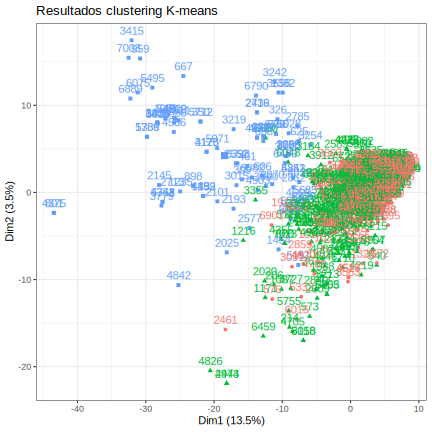
\includegraphics[width=\linewidth]{IMG/R2}
		\caption{Representación como cascada.}
		\label{fig:r2}
	\end{minipage}
\end{figure}


\newpage


\subsection{Con base en su implementación ejemplifique los conceptos de individuo,clase primitiva, clase definida, propiedad, propiedad funcional, . [30]}

\subsection{Individuo}

Dentro de la implementación, el concepto de individuo esta definido como Persona, que es la clase que representa sobre quien estamos haciendo los diagnósticos, para ello se crea la instancia juan de persona, por lo que juan es una Persona.

\subsection{Clase primitiva}

Para ejemplificar a una clase primitiva, puede tomarse el caso de la clase PersonalDeSalud la cual es general y a la que pertenecen todos aquellos que sean personal de salud que para efectos de este caso son solo la enfermera y el epidemiólogo.

\subsection{Clase definida}

El ejemplo de una clase definida es el CasoSospechoso, porque para decir que una persona es de la clase CasoSospechoso se deben pasar ciertas verificaciones lógicas, como que le Persona tenga enfermedad respiratoria y que haya viajado a un país de riesgo, esto le da pauta a pertenecer a esta clase y solamente así.

\subsection{Propiedad}

Un ejemplo de propiedad esta dado por la propiedad (o relación) presentaSintoma, la cual permite decir que una Persona instanciada como Juan, presenta un síntoma en particular como la fiebre. Nota que no es el único síntoma que puede presentar juan.

\subsection{Propiedad funcional}


Una propiedad funcional se caracteriza por tener un único valor para esa propiedad (a diferencia de la anterior con los síntomas). Un caso de este tipo de propiedades se encuentra con la propiedad funcional de resultadoLaboratorio, la cual relaciona a una persona con un resultado de laboratorio que solamente puede ser positivo o negativo, no pueden ser los 2 a la vez.


\newpage



\subsection{Ejemplifique tres metas que su ontología puede resolver [20].}

Con todo el aparato lógico, la construcción del programa y las reglas lógicas implementadas, el programa es capaz de lograr varias metas, entre ellas:

\subsubsection{Meta 1: Identificar casos}

La ontologia es capaz de identificar casos sospechosos y confirmados:

\begin{figure}[h!]
	\centering
	% Primera imagen
	\begin{minipage}[t]{0.5\linewidth} % Ajusta el ancho para la primera imagen
		\centering
		\includegraphics[width=\linewidth]{IMG/R3}
		\caption{Casos sospechoso.}
		\label{fig:r3}
	\end{minipage}%
	\hfill % Espacio entre las imágenes
	% Segunda imagen
	\begin{minipage}[t]{0.5\linewidth} % Ajusta el ancho para la segunda imagen
		\centering
		\includegraphics[width=\linewidth]{IMG/R4}
		\caption{Casos confirmados.}
		\label{fig:r4}
	\end{minipage}
\end{figure}
	
\newpage

\subsubsection{Meta 2: Inferir aislamiento}

La ontología es capaz de inferir en base al tipo de aislamiento, cual debería seguir cada persona:

\begin{figure}[h!]
	\centering
	% Primera imagen
	\begin{minipage}[t]{0.5\linewidth} % Ajusta el ancho para la primera imagen
		\centering
		\includegraphics[width=\linewidth]{IMG/R5}
		\caption{Aislamiento domiciliario.}
		\label{fig:r5}
	\end{minipage}%
	\hfill % Espacio entre las imágenes
	% Segunda imagen
	\begin{minipage}[t]{0.5\linewidth} % Ajusta el ancho para la segunda imagen
		\centering
		\includegraphics[width=\linewidth]{IMG/R6}
		\caption{Aislamiento hospitalario.}
		\label{fig:r6}
	\end{minipage}
\end{figure}

Nótese que a Maria la manda como que necesita aislamiento domiciliario, debido a que estuvo en contacto con Juan dentro de los antecedentes. Por otro lado, al preguntarle si debería tener un aislamiento hospitalario, solo muestra a Juan como candidato a ello, debido a que es un caso confirmado y con síntomas.

		
\newpage

\subsubsection{Meta 3: Inferir si es necesario el seguimiento epidemiológico por contacto}

Otra meta es preguntarse quien necesita seguimiento epidemiológico debido a que tuvo contacto con un caso confirmado.

\begin{figure}[!h]
	\centering
	\includegraphics[width=0.5\linewidth]{IMG/R7}
	\caption{Seguimiento epidemiológico}
	\label{fig:r7}
\end{figure}

Se muestra que Maria es la única que necesita seguimiento epidemiologico, esto debido a que estuvo en contacto con juan.

En todo este proceso no sale pedro, que es una tercera instancia de persona debido a que solo se sabe que es una persona pero no se tiene más información de el para poder clasificarlo como un caso sospechoso debido a que no se tiene información de contactos, viajes o síntomas, por lo que es correcto que por la forma que esta definida la ontología, no aparezca como resultado en las consultas.


\newpage


\section{Referencias}  % Sección numerada de referencias
\bibliographystyle{apalike}  % Estilo de citas (puedes cambiarlo)
\bibliography{Biblio}        % Nombre del archivo BibTeX (sin extensión)

	
\end{document}
 

